%%% Ne pas modifier jusqu'à la ligne 25
\documentclass[a4paper,12pt]{book}
\usepackage[utf8]{inputenc}
\usepackage[french]{babel}
%%\usepackage{CJK}
\usepackage{yhmath}
\usepackage[left=2cm,right=2cm,top=3cm,bottom=2cm, headheight=1.5cm,headsep=1.5cm]{geometry}
%%\usepackage{CJKutf8}
\usepackage{amsfonts}
\usepackage{mathrsfs}
\usepackage{amsmath,amsfonts,amssymb,dsfont}
\usepackage{graphicx}
\usepackage{mnsymbol}
\usepackage{subfigure}
\usepackage{enumitem}		%\enumerate-resume
\usepackage[colorlinks=true,unicode={true},hyperindex=false, linkcolor=blue, urlcolor=blue]{hyperref}
\newcommand{\myref}[1]{\ref{#1} page \pageref{#1}}

\addto\captionsfrench{\def\tablename{Tableau}}  %légendes des tableaux
\renewcommand\thesection{\Roman{section}~-~} 
\renewcommand\thesubsection{\Roman{section}.\Alph{subsection}~-~} 
\renewcommand\thesubsubsection{\Roman{section}.\Alph{subsection}.\arabic{subsubsection}~-~} 

\newcommand{\conclusion}[1]{\newline \centerline{\fbox{#1}}}

\setcounter{secnumdepth}{3}
\parindent=0pt

\usepackage{fancyhdr}
\pagestyle{fancy}

\lhead{SJTU-ParisTech} 
%%%%%%%%%%%%%%%%%%%%%%%%%%%%%%%%%%
\chead{TR14}
\rhead{Daniel 518261910024}

\begin{document}
\renewcommand{\labelitemi}{$\blacktriangleright$}
\renewcommand{\labelitemii}{$\bullet$}


\section{Notion de cohérence temporelle}
\subsection{Définition}
En pratique, aucune onde n'est monochromatique, par le modèle d'un train d'ondes, on peut définir le temps de cohérence $\tau_c$ de la source
$[\![a]\!]$
La cohérence temporelle d'une onde est liée à la largeur de bande spectrale de la source: selon l'analyse de Fourier, on a $\tau_c * \Delta f \simeq 1$
\subsection{Source à spectre distinct}
On peut également considérer 2 sources ponctuelles $S_1$ et $S_2$ confondues mais incohérentes entre elles. 
\begin{figure}[h]
    \begin{center}
    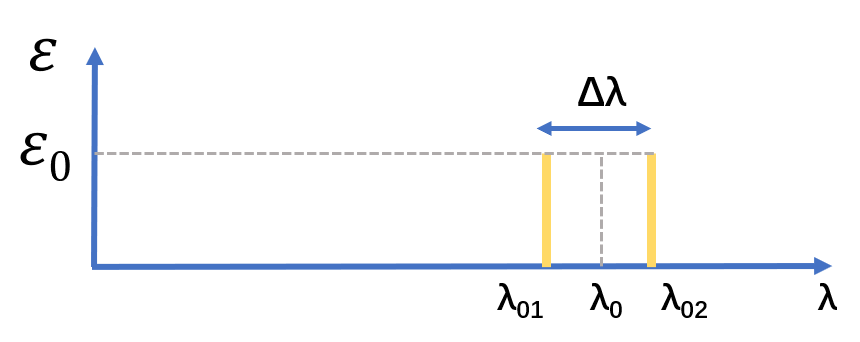
\includegraphics[scale=0.4]{tr141.png}
    \end{center}
    %\caption{Changement de densité de traits(Lazer)}
\end{figure}

On a donc au point d'observation $M$, 
\begin{align*}
    \mathcal{E}(M)&=2\mathcal{E}_1(1+\cos(\delta\varphi_1(M)))+2\mathcal{E}_2(1+\cos(\delta\varphi_2(M)))\\
    &=4\mathcal{E}_0\left[1+\cos\left(\frac{\Delta\lambda\pi\delta(M)}{\lambda_0^2}\right)\cos\left(\frac{2\pi\delta(M)}{\lambda_0}\right)\right]
\end{align*}
par les approximations que $\mathcal{E}_1=\mathcal{E}_2=\mathcal{E}_0$, et que $\lambda_0 \gg \Delta\lambda$

En posant $\mathcal{V}(\delta(M))=\cos\left(\frac{\pi\Delta\lambda\delta(M)}{\lambda_0^2}\right)$ le facteur de visibilité, on a 
$$\boxed{\mathcal{E}(M)=\mathcal{E}_{moy}(1+\mathcal{V}(\delta(M))\cos(\Delta\varphi(\delta(M)))}$$
\subsection{Source à spectre continu}
\subsubsection{densité spectrale d'éclairement à profil rectangulaire}

\begin{figure}[h]
    \begin{center}
    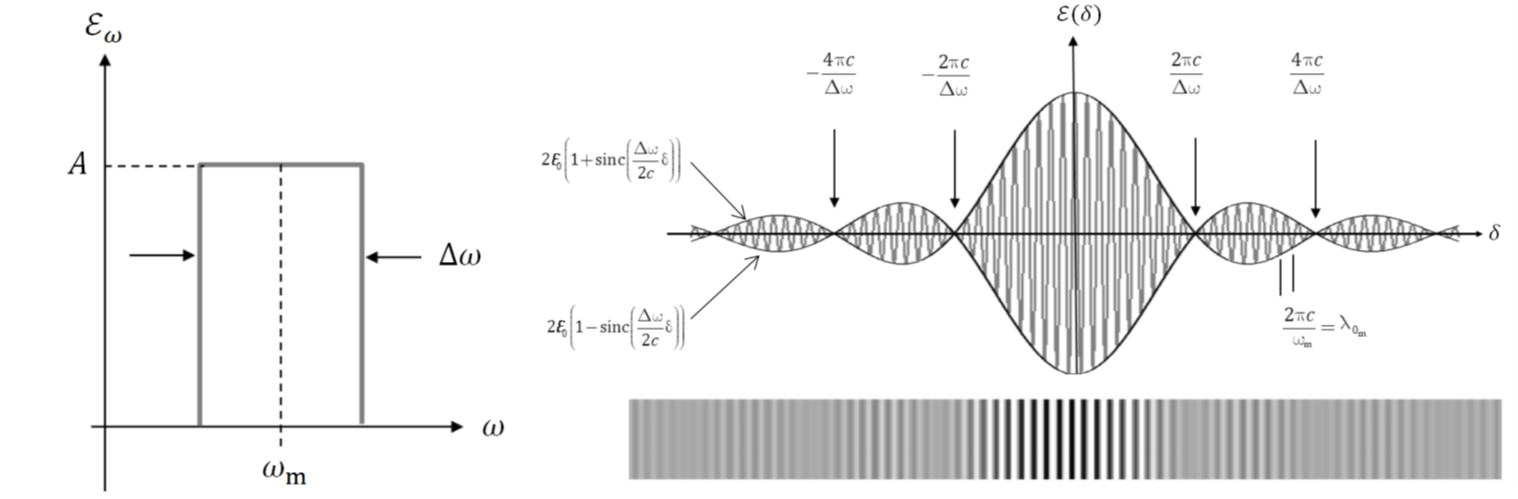
\includegraphics[scale=0.4]{tr142.png}
    \end{center}
    %\caption{Changement de densité de traits(Lazer)}
\end{figure}
On a aussi 
$$\mathcal{E}(M)=\mathcal{E}_{moy}(1+\mathcal{V}(\delta(M))\cos(\Delta\varphi(\delta(M)))$$
avec 
$\mathcal{V}(\delta(M))=sinc\left(\frac{\Delta\omega}{2c}\delta(M)\right)$

Pour une source de densité spectrale d'éclairement à profil queconque, 
le contrast $C(\delta(M))=|\mathcal{V}(\delta(M))|$ diminue globalement avec $\delta(M)$, il faut $|\delta(M)|<\frac{2\pi c}{\delta\omega}=l_c$ pour que 
les interférences soient visibles. 
\subsubsection{lumière blanche}
Dans le cas des interférences obtenues par le dispositif des deux fentes de Young, les interférences sont visibles pour 
$|x|<\frac{Dl_c}{a}$. 

Et pour les blanc d'ordre supérieure, il y a des cannelures où tous les interférences sont destructives si on utilise un prisme ou réseau,  
ces longueurs d'ondes satisfont $\lambda_m=\frac{ax}{D(m+\frac{1}{2})}$
\subsection{Interférences lumineuses à N ondes}
\begin{figure}[h]
    \begin{center}
    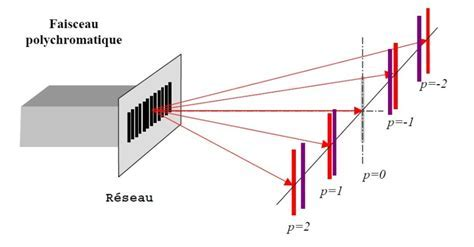
\includegraphics[scale=0.4]{tr143.jpg}
    \end{center}
    %\caption{Changement de densité de traits(Lazer)}
\end{figure}
Par la formule des réseaux, on a $\sin\theta_p=\sin\theta_0+p\frac{\lambda_0}{a}$, donc plus la longueur d'onde $\lambda$ est élevée, les lumineuses sont plus 
déviées
\subsection{Pouvoir dispersif}
Le pouvoir dispersif du réseau est défini par $P_d=\left|\frac{d\theta_p}{d\lambda_0}\right|$. Car on a $\sin\theta_p=\sin\theta_0+p\frac{\lambda_0}{a}$, 
d'où $\cos\theta_p\,d\theta_p=\frac{p}{a}\,d\lambda_0$. On a donc $P_d=\left|\frac{p}{a\cos\theta_p}\right|$
Pour augmenter $P_d$
\begin{itemize}
    \item observer en un ordre $p$ élevé
    \item utiliser un réseau de pas $a$ petit.(il ne faut pas que $a$ soit trop petit car $p\leq \lfloor\frac{a}{\lambda_0}\rfloor$)
\end{itemize}

\subsection{Recouvrement des ordres}
Pour éviter un recouvrement des ordres, il faut $\theta_{p,\lambda_{02}}<\theta_{p+1,\lambda_{01}}$, 
d'où $p<\frac{\lambda_{01}}{\lambda_{02}-\lambda_{01}}$


\subsection{Pouvoir de résolution}
\begin{figure}[h]
    \begin{center}
    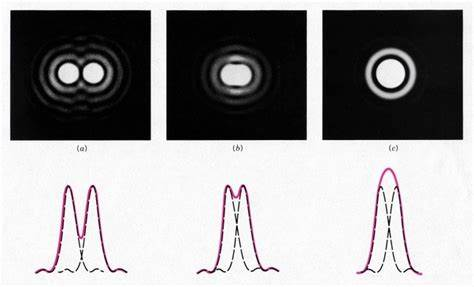
\includegraphics[scale=0.4]{tr144.jpg}
    \end{center}
    %\caption{Changement de densité de traits(Lazer)}
\end{figure}
Le plus petit écart $\Delta\lambda_{0,min}$ entre deux rayons qu'il est possible de séparer à 
l'aide d'un réseau satisfait $\frac{p\Delta\lambda_{0,min}}{a}=\frac{\lambda_0}{Na}$, soit $\Delta\lambda_{0,min}=\frac{\lambda_0}{Np}$

Le pouvoir de résolution est défini par $P_r=\frac{\lambda_0}{\Delta\lambda_{0,min}}$. On a donc $P_r=Np$
\end{document}


